\section{Einleitung und Versuchsziel}
\label{sec:aufgabenstellung}
%In der Aufgabenstellung wird (in eigenen Worten und ganzen Sätzen) formuliert, was das Ziel des 
%Versuches ist.  
%[Beachten Sie die eigentliche Aufgabenstellung in den Versuchsanleitungen sowie die Hinweise zur Auswertung!] 

Für eine Arbeit des \textsc{Polymerservice Merseburg (PSM)} wird ein temperiertes 2L-Reaktorsystem mit automatischer Dosierung über mehrere Stunden gefordert.
Mit diesem Reaktorsystem sollen testweise Polymerisationen durchgeführt werden. Somit liegt der Fokus des Systems auf der Reproduzierbarkeit der Prozesse.

Ziel des Projektes im Rahmen des Moduls Thermische Verfahrenstechnik II ist es, dass in Form einer studentischen Arbeit ein Prototyp für ein solches Reaktorsystem aufgebaut und vorgestellt wird. Die benötigten Spezifikationen an das geforderte System wurden hierfür abstrahiert und vereinfacht \mbox{(vgl. Tab. \ref{tab:Anforderungen1_2} und \ref{tab:verinfachteAnforderungen}, sowie Abb. \ref{fig:prozess 1} und \ref{fig:prozess 1_vereinfacht})}. Dabei wird aufgezeigt welche Möglichkeiten in der Umsetzung mit bereits vorhandenen Mitteln an der \textsc{Hochschule Merseburg} bestehen.

\begin{table}[h!]
	\renewcommand*{\arraystretch}{1.2}
	\centering
	%\rowcolors{2}{gray!25}{white}
	\caption{zusammengefasste Anforderungen Prozess 1 und 2}
	\label{tab:Anforderungen1_2}
	\resizebox{\textwidth}{!}{
		\begin{tabulary}{1.35\textwidth}{L|L}
			\hline
			\textbf{Anforderung} & \textbf{Beschreibung}\\
			\hline
			\rowcolor{gray!25}
			2L-Reaktor &  Es wird ein offener 2L-Reaktor für die Reaktion benötigt. \\
			Temperaturprofile & Die Temperaturen des Prozesses sind über Temperaturprofile einzustellen mit $\delta_{\text{max}}=\SI{135}{\celsius}$.\\
			\rowcolor{gray!25}
			Edukte & Es werden vorgegebene, wässrige Edukte genutzt.\\
			Ankerrührer & Für die Durchmischung ist ein Ankerrührer zu verwenden. Es darf keine Trombe entstehen.\\
			\rowcolor{gray!25}
			Stickstoffatmosphäre & Es ist eine Stickstoffschutzatmosphäre auszuführen.\\
			Wasserdampfdestillation & Es ist eine Wasserdampfdestillation auszuführen.\\
			\rowcolor{gray!25}
			Kühler & Es wird eine Kühlung ausgeführt und Kondensat in einem externen Behälter aufgefangen.\\
			pH-Wert & Für Prozess 2 ist eine pH-Wert Messung und Regelung notwendig.\\
			\rowcolor{gray!25}
			Gefriertrocknung & Für Prozess 2 ist eine Gefriertrocknung notwendig.\\
			\hline
			& Feed 1: über \SI{3}{\hour} mit \SI{135}{\milli \liter \per \hour}\\
			& Feed 2: über \SI{2}{\hour} mit \SI{500}{\milli \liter\per \hour}\\
			\multirow{-4}{*}{Feeds Prozess 1}
			& Feed 3: über \SI{4}{\hour} mit \SI{11,25}{\milli \liter \per \hour}\\
			& Feed 4: über \SI{1}{\hour} mit \SI{20}{\milli \liter \per\hour}\\
			\rowcolor{gray!25}
			\hline
			& Feed 1: über \SI{4}{\hour} mit \SI{20}{\milli \liter \per\hour}\\
			\rowcolor{gray!25}
			& Feed 2: über \SI{5}{\hour} mit \SI{6,78}{\milli \liter\per \hour}\\
			\rowcolor{gray!25}
			& Feed 3: zeitnahes Zugeben von  \SI{0,2385}{\milli \liter} unter Beachtung des Siedeverzuges\\
			\rowcolor{gray!25}
			\multirow{-3}{*}{Feeds Prozess 2 }
			& Feed 4: sekundenschnelle Zugabe von \SI{0,0555}{\milli \liter}\\
			\rowcolor{gray!25}
			& Feed 5: sekundenschnelle Zugabe von \SI{0,1223}{\milli \liter}\\
			\rowcolor{gray!25}
			& Feed 6: je nach pH-Wert Zugabe von \SI{0,0659}{\milli \liter}\\
			\hline			
	\end{tabulary}}
\end{table}%
\FloatBarrier

\begin{table}[h!]
	\renewcommand*{\arraystretch}{1.2}
	\centering
	\rowcolors{2}{gray!25}{white}
	\caption{Projektanforderungen: Vereinfachung des Prozesses 1}
	\label{tab:verinfachteAnforderungen}
	\resizebox{\textwidth}{!}{
		\begin{tabulary}{1.35\textwidth}{L|L}
			\hline
			\textbf{Anforderung} & \textbf{Beschreibung}\\
			\hline
			2L-Reaktor &  Es wird ein offener 2L-Reaktor für die Reaktion benötigt. \\
			Temperaturprofile & Die Temperaturen des Prozesses sind über Temperaturprofile einzustellen mit $\delta_{\text{max}}=\SI{80}{\celsius}$.\\
			Feed 1 zu dosieren & Feed 1 ist mit \SI{135}{\milli \liter \per \hour} über \SI{3}{\hour} zuzudosieren.\\
			Feed 4 zu dosieren & Feed 4 ist mit \SI{20}{\milli \liter \per \hour} über \SI{1}{\hour} zuzudosieren.\\
			Feed 3 \& Feed 4 & Feed 3 und 4 werden nicht ausgeführt.\\
			Edukte & Wasser wird als Ersatz für die realen Edukte genutzt.\\
			Ankerrührer & Für die Durchmischung ist ein Ankerrührer zu verwenden. Es darf keine Trombe entstehen.\\
			Stickstoffatmosphäre & Es wird keine Schutzatmosphäre ausgeführt.\\
			Wasserdampfdestillation & Es wird keine Wasserdampfdestillation ausgeführt.\\
			Kühler & Es wird keine Kühlung ausgeführt und kein Kondensat aufgefangen.\\
			\hline			
	\end{tabulary}}
\end{table}%
\FloatBarrier

\begin{figure}
	\centering
	\begin{minipage}{.5\textwidth}
		\centering
		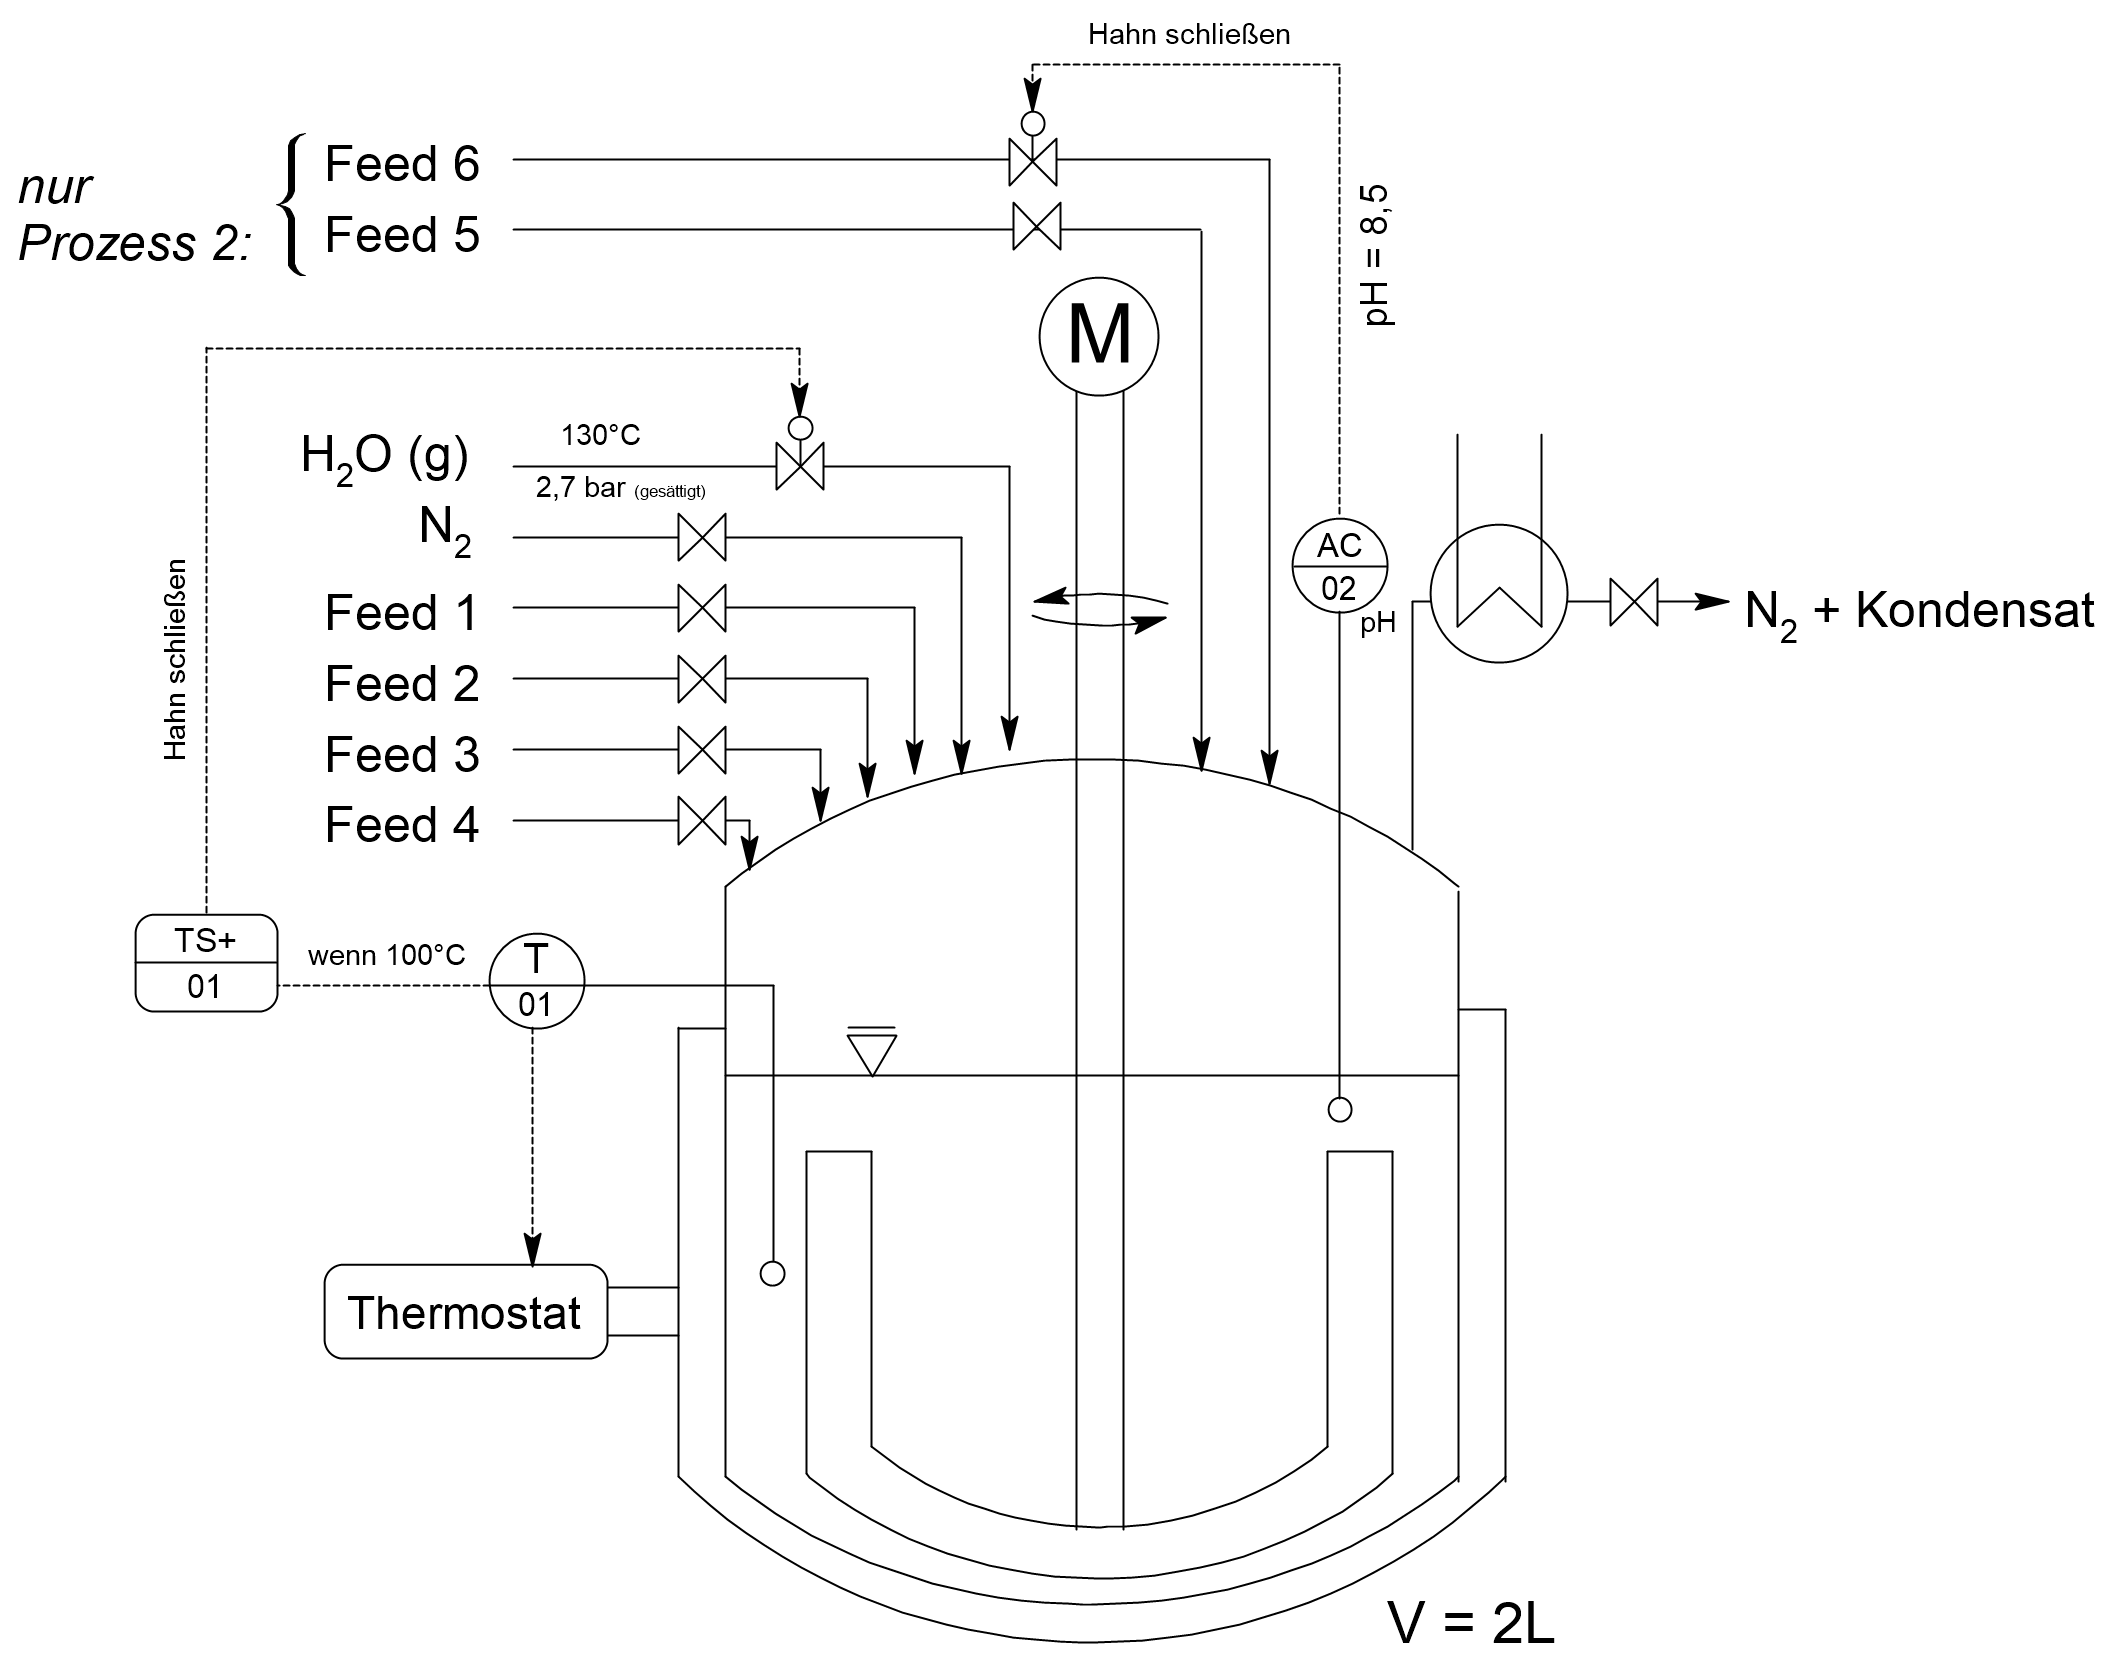
\includegraphics[width=0.8\linewidth]{img/Skizze_Prozess_gesamt.png}
		\captionof{figure}{Skizze der realen Anforderungen an das Reaktorsystem}
		\label{fig:prozess 1}
	\end{minipage}%
	\hfill
	\begin{minipage}{.45\textwidth}
		\centering
		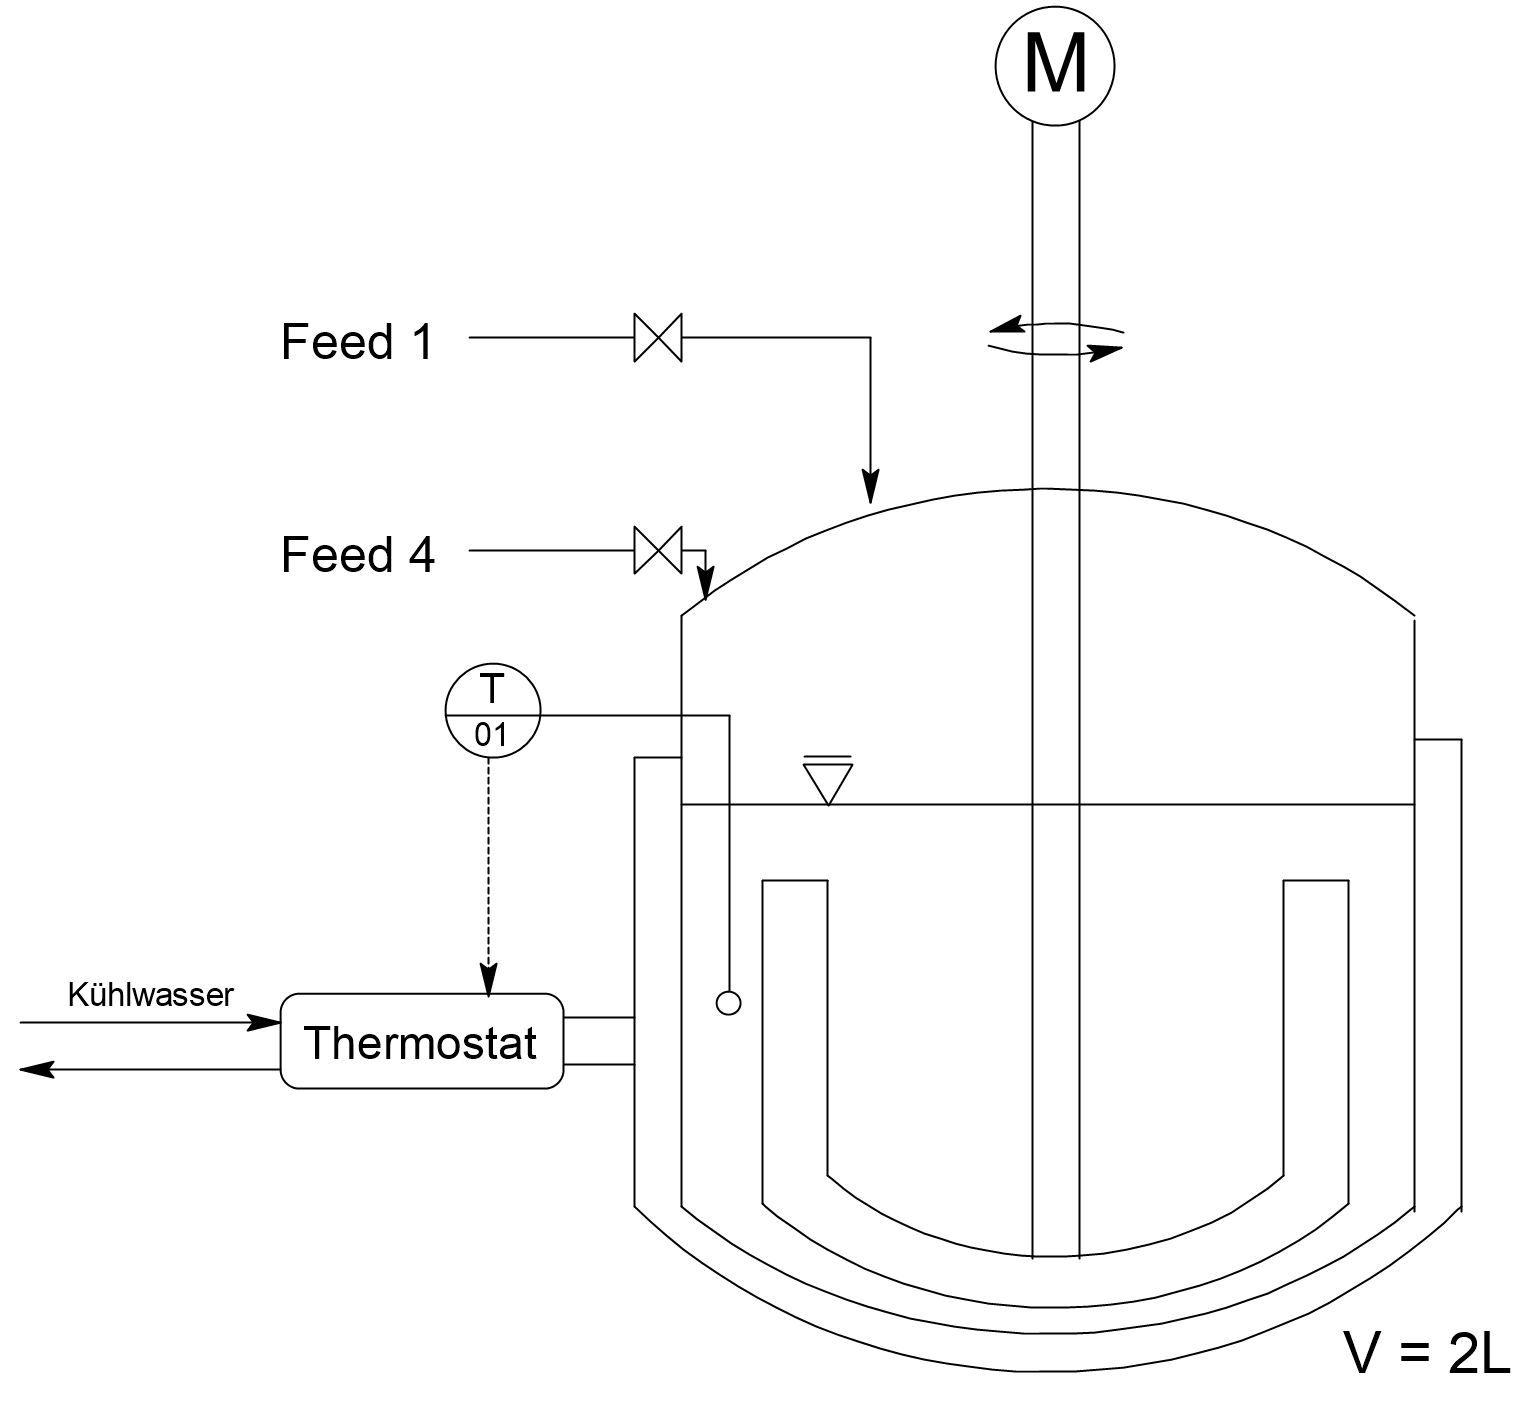
\includegraphics[width=0.75\linewidth]{img/Skizze_Prozess_1_vereinfacht.png}
		\captionof{figure}{Skizze der vereinfachten Anforderungen an das Reaktorsystem für Prozess 1}
		\label{fig:prozess 1_vereinfacht}
	\end{minipage}
\end{figure}